\documentclass[tikz,border=10pt]{standalone}
\usepackage{tkz-euclide} % 专门用于简化几何作图的宏包

\begin{document}
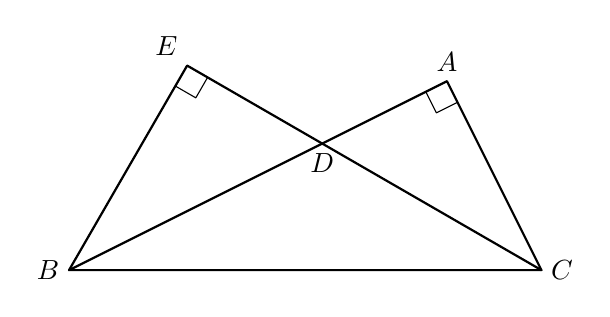
\begin{tikzpicture}[line cap=round, line join=round, >=stealth, scale=1.5]
    % 1. 定义核心顶点坐标 (基于图像比例进行参数化设置)
    \coordinate (B) at (0,0);
    \coordinate (C) at (4,0);
    
    % 定义角EBC和角ACB的近似角度以还原图形形状
    % E点满足 BE 垂直 EC (即在以BC为直径的圆上)
    \coordinate (E) at (1, 1.732); 
    % A点满足 BA 垂直 AC (即在以BC为直径的圆上)
    \coordinate (A) at (3.2, 1.6);

    % 2. 计算交点 D (线段 AB 和 EC 的交点)
    \coordinate (D) at (intersection of B--A and E--C);

    % 3. 绘制主要轮廓线
    \draw[thick] (B) -- (C) -- (A) -- (B); % 绘制三角形 ABC
    \draw[thick] (B) -- (E) -- (C);       % 绘制线段 BE, EC

    % 4. 绘制直角标记
    % 标记角 BAC 为直角
    \tkzMarkRightAngle[size=0.2](B,A,C)
    % 标记角 BEC 为直角
    \tkzMarkRightAngle[size=0.2](B,E,C)

    % 5. 标注顶点文字
    % anchor 用于微调文字位置，确保不与线段重叠
    \node[left] at (B) {$B$};
    \node[right] at (C) {$C$};
    \node[above left] at (E) {$E$};
    \node[above] at (A) {$A$};
    \node[below] at (D) {$D$};

\end{tikzpicture}
\end{document}